% Number 70
% Vectors UFPM
% Component of mg parallel to plane?
% MIT Physics for Teachers LON-CAPA

% Watermark
\AddToShipoutPicture*{\BackgroundPic}

\addtocounter {ProbNum} {1}

\begin{floatingfigure}[r]{.25\textwidth}
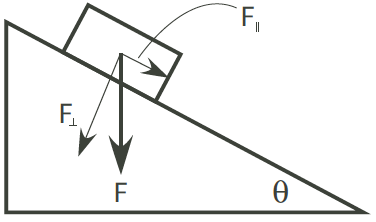
\includegraphics[scale=.4]{/Users/jgates/desktop/latex/pics/inclinedplane2.png}
\end{floatingfigure}
 
{\bf \Large{\arabic{ProbNum}}} A gravitational force of magnitude F acts vertically downward on a block resting on a plane. The plane makes an angle of $\theta$ with the horizontal. 

\bigskip

\indent What is the magnitude of the component of the gravitational force acting parallel to the plane? 

\vfill

\newpage
